
\chapter{La mise en \oe{}uvre de l'API}
\label{implementation.chap}


\GT{Avant d'avoir une subsection, tu dois avoir une section. Donc, v\'erifie la structure de ce chapitre!}

\subsection{Pipeline}

Tel que mentionn\'e au chapitre pr\'ec\'edent, un pipeline est compos\'e d'une cha\^ine de traitement appel\'e \TT{Pipe}. Un \TT{Pipe} est repr\'esent\'e essentiellement par une s\'erie d'op\'erateurs d\'efinis par l'utilisateur qui sont appliqu\'es aux \'el\'ements d'un flux. \TT{PpFf} est impl\'ement\'e au-dessus de la biblioth\`eque \TT{FastFlow}, de sorte que nous utilisons les constructions \TT{ff\_node}, \TT{ff\_pipeline} et \TT{ff\_farm} de \TT{FastFlow} pour l'ex\'ecution de \TT{PpFf}. 

Tels que d\'ecrits au chapitre pr\'ec\`edent, les op\'erateurs qui composent un \TT{Pipe} sont de deux types : les op\'erateurs sans \'etat et les op\'erateurs avec \'etat. Comme on peut le voir dans la figure~\ref{MapToFastFlow.fig}, un op\'erateur h\'erite de la class \TT{ff\_node} de \TT{FastFlow}. Un \TT{Pipe} contient un ou plusieurs op\'erateurs sans \'etat et un seul op\'erateur avec \'etat. Lorsque ce dernier est ajout\'e dans le \TT{pipeline}, la m\'ethode \TT{run()} est appel\'ee. \`A ce stade, un objet de type \TT{ff\_pipeline} correspondant au \TT{Pipe} est cr\'e\'e. Ensuite, chaque op\'erateur d\'efini par l'utilisateur est visit\'e et en fonction de la configuration \'etablie, des objets de type \TT{ff\_node} ou \TT{ff\_farm} sont ajout\'es comme stage au \TT{ff\_pipeline}. Chaque nœud ainsi ajout\'e dans \TT{ff\_pipeline} sera ex\'ecut\'e dans un fil d'ex\'ecution.
La cr\'eation de \TT{Pipe} est r\'ealis\'ee \`a l'aide de \TT{PipeManager}.

\begin{figure}[ht]
\centering
     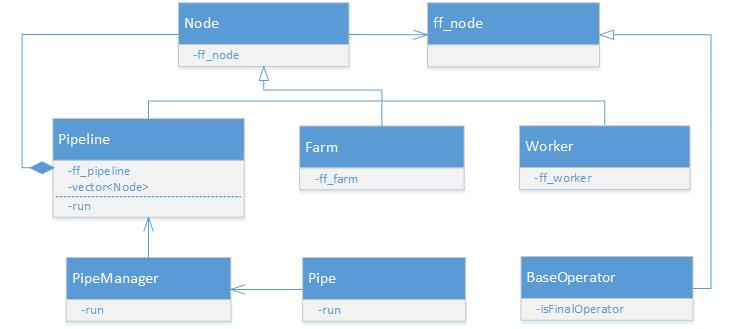
\includegraphics[width=1.0\textwidth]{Figures/MapToFastFlow.jpg}
      \caption{La correspondance entre les \'el\'ements de \TT{PpFf} et ceux de  \TT{FastFlow}.}
       \label{MapToFastFlow.fig}
\end{figure}


\subsection{Parall\'elisation}

La cr\'eation de code parall\`ele est g\'en\'eralement consid\'er\'e du domaine d'experts. La complexit\'e du code parall\`ele diminue la productivit\'e, ce qui peut augmenter les co\^uts de d\'eveloppement. \TT{PpFf} permet aux programmeurs de composer du code s\'equentiel et de l'ex\'ecuter en parall\`ele. Par l'interm\'ediaire d'une interface unique, l'API offre deux mod\`eles de parall\'elisme : le parall\'elisme de flux et \TT{Task-Farm}.

\GT{Si tu parles de <<parall\'elisme de flux>>, alors tu devrais
parler de <<parall\'elisme de t\^aches>>, ou <<parall\'elisme de
donn\'ees>>. Un Task-Farm est un m\'ecanisme sp\'ecifique pour mettre
en oeuvre une de ces deux derni\`eres formes de parall\'elisme.}


\subsubsection{Parall\'elisme de flux}

Le parall\'elisme de flux consiste \`a ex\'ecuter plusieurs \'etapes d'un traitement s\'equentiel en parall\`ele en leur faisant traiter des données diff\`erentes. Les donn\'ees se succ\`edent ainsi les unes aux autres dans les diff\'erentes \'etapes --- appel\'ees  aussi des \emph{stages}. \`A noter que ce type de parall\'elisme est appliqu\'e par d\'efaut dans notre API. Le traitement effectu\'e dans un \emph{stage} un instant donn\'e peut d\'ependre des traitements effectu\'es par ce m\^eme \emph{stage} pour les donn\'ees pr\'ec\'edentes --- un \'etat interne est donc conserv\'e. Ce fonctionnement permet de parall\'eliser des traitements avec de fortes d\'ependances entre les donn\'ees sans avoir recours \`a de nombreuses synchronisations. 
Un flux avec $n$ \emph{stages} peut \^etre formellement exprim\'e sous la forme d'une composition s\'equentielle d'op\'erateurs sur les \'el\'ements d'entr\'ee comme suit~: 

\[
	O(x) = O_n( \ldots (O_k( \ldots O_1(x)) \ldots ) \ldots ));
\]

Dans ce cas, le parall\'elisme est repr\'esent\'e par un graphe lin\'eaire de $n$ travailleurs. Chaque travailleur correspond \`a une op\'eration sp\'ecifique. La figure~\ref{ParallelismeDuFlux.fig} montre la repr\'esentation graphique du parall\'elisme de flux. Cette solution n'acc\'el\`ere pas le calcul d'un seul \'el\'ement. Par contre, elle am\'eliore le d\'ebit de sortie.

\GT{Si tu as une figure, alors tu dois y r\'ef\'erer dans le texte.}

\GT{Il faudrait expliquer, dans la figure, \`a quoi correspondent
$S_i$ et $W_i$.}

\begin{figure}[ht]
\centering
     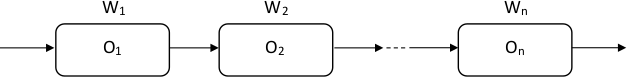
\includegraphics[width=1.0\textwidth]{Figures/ParallelismeDuFlux.jpg}
      \caption{Une repr\'esentation graphique du parall\'elisme de flux pour une d\'ecomposition en $n$ \emph{stages} $O_1, O_2, \ldots, O_n$.}
       \label{ParallelismeDuFlux.fig}
\end{figure}


\subsubsection{Parall\'elisme de donn\'ees et \emph{Task Farm}}

\GT{Donc, sur la base de la description que tu donnes ci-bas, il
s'agit de <<parall\'elisme de donn\'ees>>. C'est ce qu'il faut
indiquer un peu partout. Par contre, tu peux ensuite indiquer que ce
parall\'elisme de donn\'ees est mis en oeuvre avec un Task Farm de
FastFlow.}

Le parall\'elisme de donn\'ees impl\'ement\'e dans \TT{PpFf}  consiste \`a r\'epliquer un op\'erateur parmi un ensemble de travailleurs identiques. Autrement dit, il vise \`a effectuer un traitement identique sur un ensemble de donn\'ees ind\'ependantes les unes des autres. 
%
Dans notre impl\'ementation de \PpFf, le parall\'elisme de donn\'ees est mis en oeuvre avec les \emph{Task Farm} de FastFlow.


\GT{Bon, je crois que le probl\`eme ici, qui rend l'explication
compliqu\'ee, c'est que tu n'as pas d\'ecrit FastFlow.  Il faudrait
que, dans un chapitre pr\'ec\'edent, tu expliques FastFlow, notammen
\TT{ff\_farm}. Ensuite, ici, tu pourrais simplement r\'ef\'erer \`a
ces explications ant\'erieures.}

Une instance de \TT{Task-Farm} est compos\'ee de trois principales entit\'es : un \TT{Emitter}, un \TT{Collector} et de multiples instances de travailleurs. L'\TT{Emitter} distribue les \'el\'ements d'entr\'ee aux travailleurs selon une certaine politique d'ordonnancement afin d'\'equilibrer la charge des travailleurs. La figure~\ref{ParallelismeTaskFarm.fig} montre le mod\`ele \emph{TaskFarm} tel qu'utilis\'e dans \TT{PpFf}. Par d\'efaut, les \'el\'ements sont repartis aux divers travailleurs selon une politique \emph{round robin}. Les travailleurs re\c{c}oivent les \'el\'ements d'entr\'ee et appliquent sur chacun d'eux l'op\'erateur d\'efini au pr\'ealable par l'utilisateur. Les r\'esultats sont envoy\'es vers le \TT{Collector} charg\'e de les collecter --- i.e., de les combiner --- puis de les transmettre au flux de sortie.

Dans \TT{PpFf}, les \'el\'ements du flux sont trait\'es dans l'ordre d'arriv\'ee selon le principe \emph{FIFO}. La collection de plusieurs r\'esultats \`a l'aide de cette approche r\'esulte dans un flux sans ordre sur ses \'el\'ements. En effet, le \TT{Collector} transmet les \'el\'ements au flux de sortie dans l'ordre d'arriv\'ee. \'Etant donn\'e que plusieurs flux ind\'ependants sont impliqu\'es, cet ordre ne peut pas \^etre pr\'ed\'etermin\'e. Si le respect d'un  ordre sp\'ecifique est requis, l'utilisateur de l'API peut ajouter un op\'erateur qui produit cet ordre --- \GT{par ex., l'op\'erateur ???}.

L'impl\'ementation parall\`ele de ce mod\`ele peut \^etre formellement
exprim\'ee sous la forme d'un ensemble de travailleurs $WS$ qui
applique l'op\'erateur $O$ sur les \'el\'ements $X$ apparaissant dans
le flux d'entr\'ee~:

\[
	WS = {W_1, W_2,\ldots, W_n}
\]

\[
	O : X \rightarrow Y
\]

Le r\'esultat $Y_i$ est g\'en\'er\'e en appliquant l'op\'erateur $O$ sur l'\'el\'ement $X_i$. L'op\'eration sera ex\'ecut\'ee en parall\`ele par les diff\'erents travailleurs. Dans ce cas, la structure du mod\`ele d'ex\'ecution peut \'eventuellement recevoir, en param\`etre, le nombre de travailleurs \`a utiliser pour l'ex\'ecution parall\`ele. Si ce param\`etre n'est pas sp\'ecifi\'e, un seul travailleur est activ\'e. Cette solution de permettre d'augmenter le nombre de travailleurs permet d'augmenter le d\'ebit du traitement des donn\'ees, c'est-\`a-dire le nombre de donn\'ees qui peuvent \^etre trait\'ees en un temps donn\'e.

\begin{figure}[ht]
\centering
     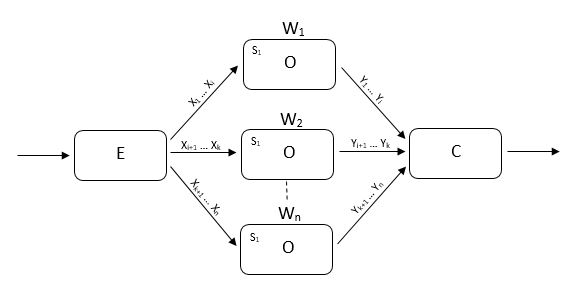
\includegraphics[width=1.0\textwidth]{Figures/ParallelismeTaskFarm.jpg}
      \caption{Un \emph{Task Farm} de FastFlow.}
       \label{ParallelismeTaskFarm.fig}
\end{figure}




\subsection{Stages}

\GT{A relire}

Le traitement en parall\`ele d'un flux de donn\'ees contribue \`a augmenter les performances du pipeline en utilisant les cœurs de la machine. Cependant, il existe une limitation lorsque le parall\'elisme est appliqu\'e sur certains op\'erateurs. Dans \PpFf, seuls les op\'erateurs sans \'etat peuvent \^etre parall\'elis\'es en toute s\'ecurit\'e. Par contre, quand il est n\'ecessaire de parall\'eliser un op\'erateur avec \'etat, les choses deviennent un peu plus compliqu\'ees parce que les r\'esultats du calcul sont obtenus en traitant un ensemble d'\'el\'ements d'entrée appartenant \'a un ou plusieurs flux de donn\'ees. Comme la plupart des traitements consistent en une combinaison d'op\'erateurs avec ou sans \'etat, un traitement parall\`ele ne peut pas \^etre effectu\'e. Une solution consiste alors \`a parall\'eliser les op\'erateurs sans \'etat et \`a utiliser un op\'erateur \TT{Collector} pour fusionner les flux parall\`eles avant d'appliquer un op\'erateur avec \'etat. Cette solution implique l'utilisation d'un autre cœur de la machine. De plus, le traitement pour les op\'erateurs avec \'etat est effectu\'e de fa\c{c}on s\'equentielle. Afin d'optimiser le traitement, nous avons introduit les \emph{stages}.

Un \emph{stage} repr\'esente le groupement logique d'un ou plusieurs op\'erateurs d'une \'etape dans la cha\^ine de traitement d'un pipeline. La figure (\`a ajouter la r\'ef\'erence stage.fig) montre plusieurs op\'erateurs finaux group\'es logiquement dans un stage.  \`A noter que ce module n'est pas visible \`a l'utilisateur. Dans \TT{PpFf}, nous distinguons deux types de \emph{stages} : les \emph{stages} interm\'ediaires et les \emph{stages} finaux. Comme leur nom le sugg\`ere, les \emph{stages} interm\'ediaires groupent seulement les op\'erateurs sans \'etat et les \emph{stages} finaux groupent les op\'eateurs finaux. Dans le cas du traitement parall\`ele, les \emph{stages} finaux ont le r\^ole de r\'eduire l'\'etat d'op\'erateurs finaux de chaque fil d'ex\'ecution selon l'op\'eration donn\'ee. La valeur issue repr\'eente le r\'esultat du traitement du flux de donn\'ees.



